\documentclass{beamer}
\usepackage[utf8]{inputenc}

\usetheme{Madrid}
\usecolortheme{default}
\usepackage{txfonts}
\usepackage{listings}
\usepackage{adjustbox}
\usepackage{tabularx}
\usepackage{lmodern}
\usepackage{circuitikz}
\usepackage{tikz}

\usepackage{gvv}
\usepackage{cite}
\usepackage{amsmath,amssymb,amsfonts,amsthm}
\usepackage{algorithmic}
\usepackage{graphicx}
\usepackage{textcomp}
\usepackage{xcolor}
\usepackage{txfonts}
\usepackage{listings}
\usepackage{enumitem}
\usepackage{mathtools}
\usepackage{gensymb}
\usepackage{comment}
\usepackage{tkz-euclide} 
\usepackage{listings}                                      
\def\inputGnumericTable{}                                
\usepackage{color}                                            
\usepackage{array}                                            
\usepackage{longtable}
\usepackage{multicol}
\usepackage{calc}                                             
\usepackage{multirow}                                         
\usepackage{hhline}                                           
\usepackage{ifthen}

\setbeamertemplate{page number in head/foot}[totalframenumber]

\usepackage{tcolorbox}
\tcbuselibrary{minted,breakable,xparse,skins}



\definecolor{bg}{gray}{0.95}
\DeclareTCBListing{mintedbox}{O{}m!O{}}{%
  breakable=true,
  listing engine=minted,
  listing only,
  minted language=#2,
  minted style=default,
  minted options={%
    linenos,
    gobble=0,
    breaklines=true,
    breakafter=,,
    fontsize=\small,
    numbersep=8pt,
    #1},
  boxsep=0pt,
  left skip=0pt,
  right skip=0pt,
  left=25pt,
  right=0pt,
  top=3pt,
  bottom=3pt,
  arc=5pt,
  leftrule=0pt,
  rightrule=0pt,
  bottomrule=2pt,
  toprule=2pt,
  colback=bg,
  colframe=orange!70,
  enhanced,
  overlay={
    \begin{tcbclipinterior}
    \fill[orange!20!white] (frame.south west) rectangle ([xshift=20pt]frame.north west);
    \end{tcbclipinterior}},
  #3,
}
\lstset{
    language=python,
    basicstyle=\ttfamily\small,
    keywordstyle=\color{blue},
    stringstyle=\color{orange},
    commentstyle=\color{green!60!black},
    numbers=left,
    numberstyle=\tiny\color{gray},
    breaklines=true,
    showstringspaces=false,
}

\title 
{3.0.31}
\date{}


\author 
{Sai Sreevallabh - EE25BTECH11031}



\begin{document}

\frame{\titlepage}

\begin{frame}{Question:}
If $X$ is a continuous random variable whose probability density function is given by
       $$
f(x) =
\begin{cases}
K\brak{5x - 2x^2}, & 0 \leq x \leq 2, \\
0, & \text{otherwise}.
\end{cases}
$$
 Then $P(X>1)$ is
    % \begin{enumerate}
    %             \item 3/14
    %             \item 4/5
    %             \item 14/17
    %             \item 17/28
    % \end{enumerate}
    
\end{frame}

\begin{frame}{Theoretical Solution}

For $f(x)$ to be a valid pdf, it must satisfy the property
\begin{align*}
    \int_{-\infty}^{\infty} f(x) \, dx = 1\\
    \implies K \int_{0}^{2} (5x - 2x^2) \, dx = 1
\end{align*}

This gives the value of K as $\boxed{K = \frac{3}{14}}$
    
\end{frame}

\begin{frame}{Theoretical Solution}

Using the above obtained value of K, we can find the desired probability $P\brak{X>1}$.

\begin{align*}
P(X > 1) &= \int_{1}^{\infty} f(x) \, dx \\
&= \int_{1}^{2} \frac{3}{14} \brak{5x - 2x^2} \, dx \\
&= \frac{3}{14} \sbrak{\frac{5x^2}{2} - \frac{2x^3}{3}}_1^2 \\
& = \frac{17}{28}
\end{align*}

$\therefore \boxed{P\brak{X>1} = \frac{17}{28}}$ 
    
\end{frame}

\begin{frame}[fragile]
\frametitle{Simulation Code}

\begin{lstlisting}
import numpy as np
import matplotlib.pyplot as plt
from scipy.stats import rv_continuous
import sympy as sp

#Using SymPy to get the functions
x_sym = sp.Symbol('x')
t = sp.Symbol('t')

pdf_expr = sp.Rational(3, 14) * (5*x_sym - 2*x_sym**2)
cdf_expr = sp.integrate(pdf_expr.subs(x_sym, t), (t, 0, x_sym))

# Convert to fast numerical functions
pdf_num = sp.lambdify(x_sym, pdf_expr, 'numpy')
cdf_num = sp.lambdify(x_sym, cdf_expr, 'numpy')

\end{lstlisting}

    
\end{frame}

\begin{frame}[fragile]
\frametitle{Simulation Code}

\begin{lstlisting}
#SciPy
class CustomDist(rv_continuous):
    def _pdf(self, x):
        return pdf_num(x)
    
    def _cdf(self, x):
        return cdf_num(x)

my_dist = CustomDist(a=0, b=2, name='fully_automated')
x_vals = np.linspace(-0.5, 3, 500)
x_shade = np.linspace(1, 2, 100)

#Plotting pdf
plt.plot(x_vals, my_dist.pdf(x_vals), color='blue', lw=2, label='$f(x)$')
plt.fill_between(x_shade, my_dist.pdf(x_shade), color='skyblue', alpha=0.5, label='P(X > 1)')
plt.axvline(1, color='red', linestyle='--', alpha=0.5)

\end{lstlisting}

    
\end{frame}

\begin{frame}[fragile]
\frametitle{Simulation Code}

\begin{lstlisting}
plt.xlabel('x')
plt.ylabel('f(x)')
plt.grid(True, alpha=0.3)
plt.legend()
plt.tight_layout()
plt.savefig("Figs/pdf.png")
plt.show()

#Plotting CDF for verification
plt.plot(x_vals, my_dist.cdf(x_vals), color='green', lw=2, label='CDF')

p_le_1 = my_dist.cdf(1)
plt.scatter([1], [p_le_1], color='red', zorder=5)

\end{lstlisting}

    
\end{frame}

\begin{frame}[fragile]
\frametitle{Simulation Code}

\begin{lstlisting}
plt.annotate(f'P(X \u2264 1) = {p_le_1:.4f}\n(11/28)', 
             (1, p_le_1), textcoords="offset points", xytext=(-40,15), ha='center',
             bbox=dict(boxstyle="round,pad=0.3", fc="white", ec="gray", lw=1))

plt.axvline(1, color='red', linestyle='--', alpha=0.5)
plt.axhline(p_le_1, color='red', linestyle='--', alpha=0.5)

plt.xlabel('x')
plt.ylabel('F(x)')
plt.grid(True, alpha=0.3)
plt.legend()
plt.tight_layout()
plt.savefig("Figs/cdf.png")
plt.show()

\end{lstlisting}    
\end{frame}

\begin{frame}{Simulation Plots}

\begin{figure}
    \centering
    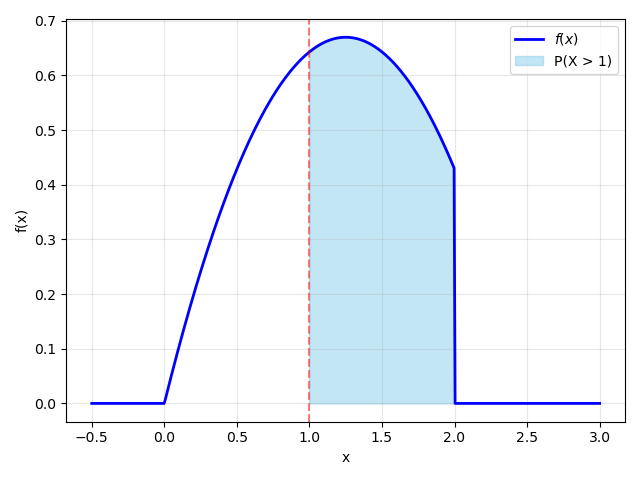
\includegraphics[width=0.95\linewidth]{Figs/pdf.png}
\end{figure}
    
\end{frame}

\begin{frame}{Simulation Plot}

\begin{figure}
    \centering
    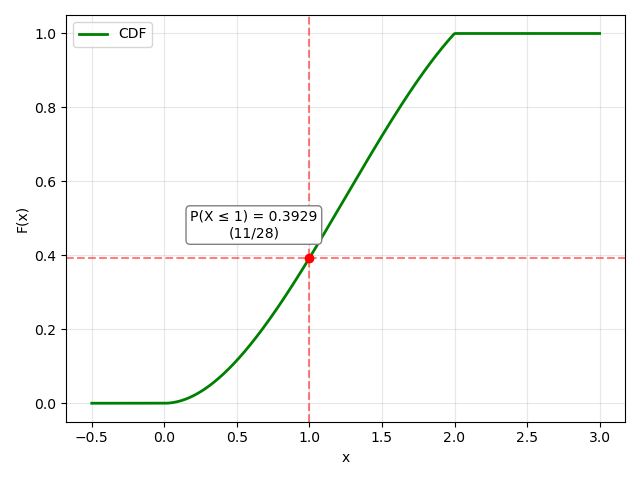
\includegraphics[width=0.95\linewidth]{Figs/cdf.png}
\end{figure}
    
\end{frame}

\end{document}

\end{document}

